% !TEX root = SADR.tex
\section{Proposed Method}
We first provide an overview of the proposed \ours {} approach to model user and item homophily via attention based nets while also modeling temporal relations. We subsequently discuss the details of each employed module.

\subsection{Overall Architecture}
Our goal is to create a ranked list of items, indicating the preference of a user $u$ for interacting with item $i\in{\mathcal I}$ at time $t$. Here, ${\mathcal I}$ represents the set of all items available on the considered platform. We compute this ranked list by sorting probability scores $\hat{r}_{u,i}^{t}$ for a user $u$ and item $i$ at time $t$. Formally, given user $u$ and time $t$
we obtain $\forall i$,  the probability scores  after scaling the output of a linear layer, i.e.,
\begin{align}
  \hat{r}_{u,i}^{t} &= \sigma \left(\lambda_1S_1 + \lambda_2S_2 + \lambda_3S_3+\lambda_4S_4+ b_c\right).
  \label{eq:fuse}
\end{align}
Hereby $\sigma$ denotes the sigmoid function, $b_c$ is a learnable bias, and $\lambda_k\in\mathbb{R}$, $k\in\{1, \ldots, 4\}$, are four learnable weights for the scores $S_k$. Importantly, because we learn a linear combination of scores, we are able to study their magnitude which provides %interpretable
evidence regarding the importance of the different factors in the proposed \ours {} model. See \Cref{sec:mod} for our experimental results.

\begin{figure}[th]
  \centering
  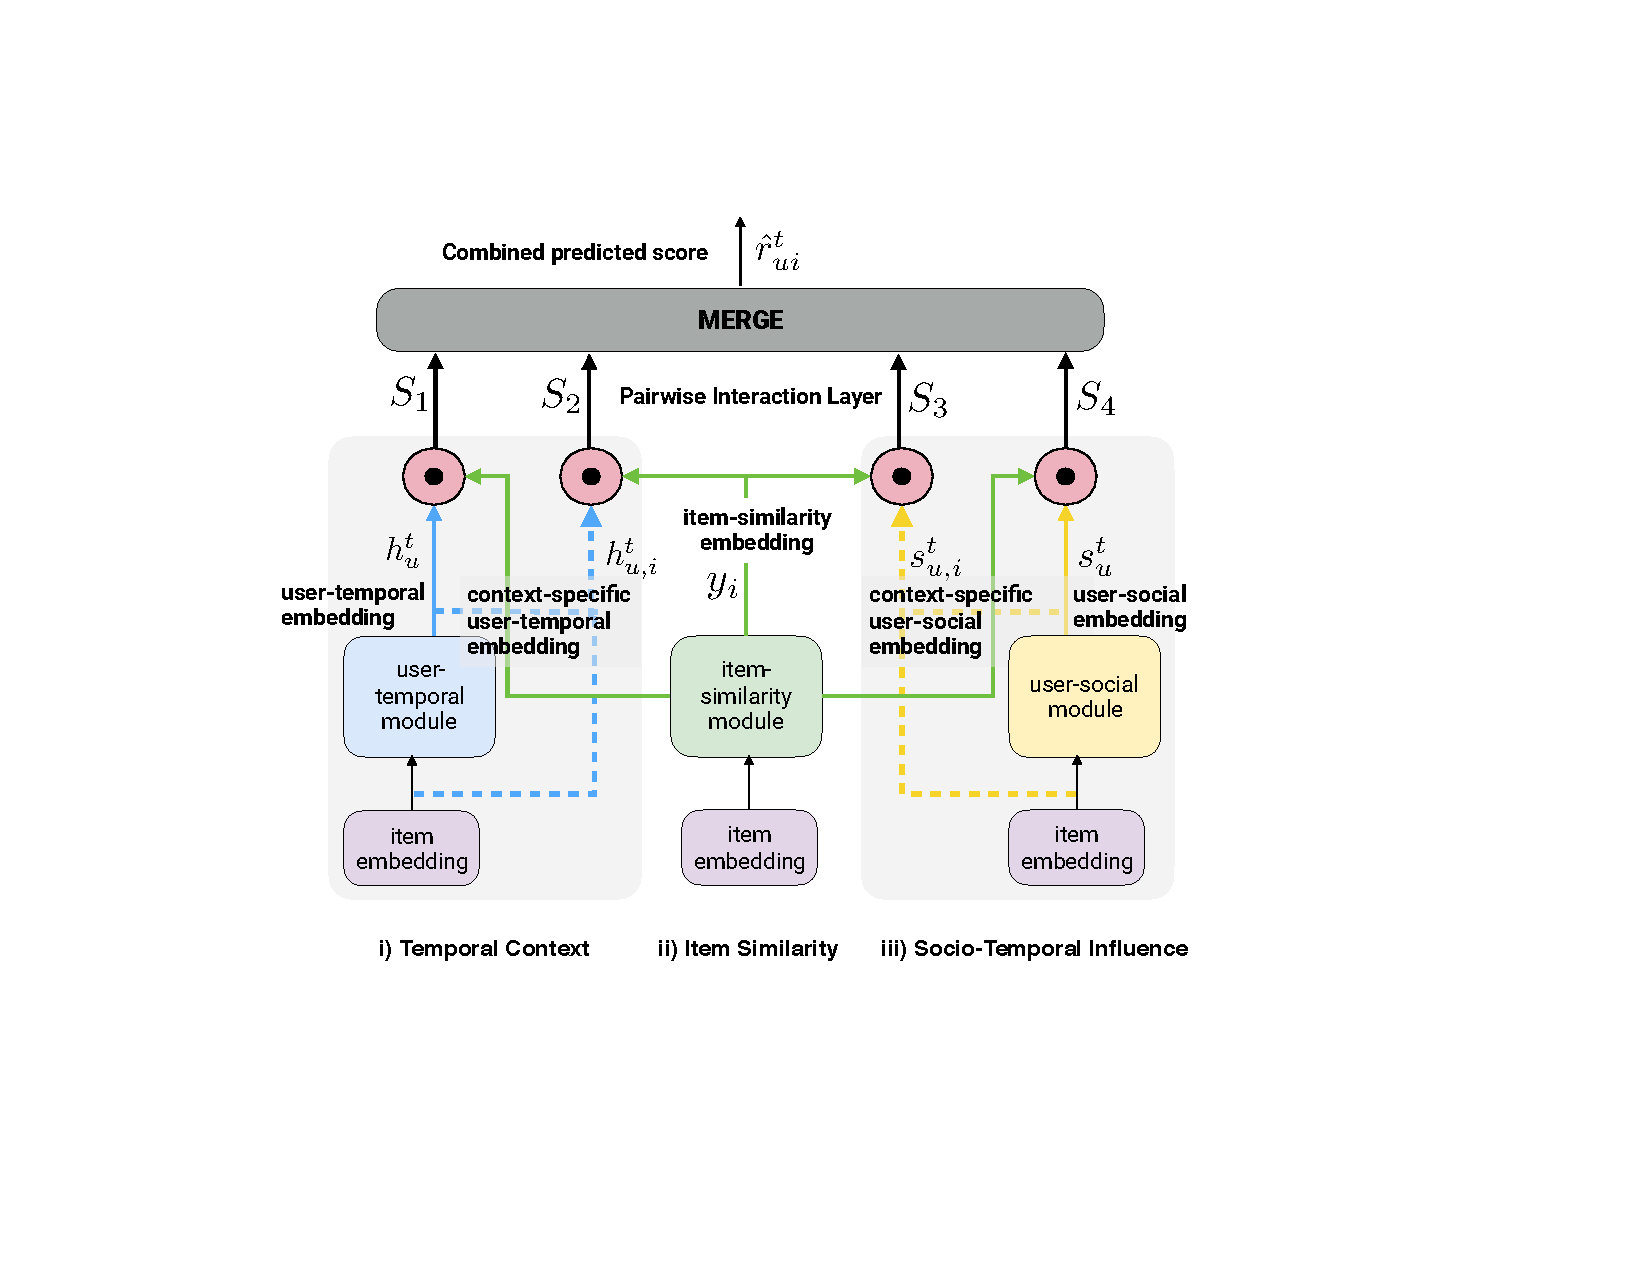
\includegraphics[width=0.7\textwidth]{figures/Overall_new}
  \caption{Overview of the proposed \ours {} model.  Our model computes pairwise interaction scores which compares item embeddings from the item-similarity module with user embeddings from both the user-temporal module and the user-social module. These scores are then merged using learnable weights to compute the final predicted score.
  }
  \label{fig:overview}
\end{figure}

As illustrated in Figure~\ref{fig:overview}, we obtain the  scores $S_k$ by combining information from the following three modules:
(1) the user-temporal module which leverages temporal information about a user;
(2) the user-social module which captures information about the recent interactions of a user's friends; and
(3) the item-similarity module, which captures information about item homophily.

Specifically, Eq.~\eqref{eq:fuse} combines four  pairwise interactions:
(1) $S_1 = h_u^{t} \cdot {y}_i$,
(2) $S_2 = h_{u, i}^{t} \cdot {y}_i$,
(3) $S_3 = s_u^{t} \cdot {y}_i$, and
(4) $S_4 = s_{u, i}^{t} \cdot {y}_i$.
Hereby, $\cdot$ indicates an inner product between two embeddings.
Note, all pairwise interaction scores $S_k$ assess the similarity between a $D$-dimensional representation obtained from the item-similarity module (${y}_i\in\mathbb{R}^D$) and information obtained from either the user-temporal module ($h_u^{t} , h_{u,i}^{t}\in\mathbb{R}^D$) or the user-social module ($s_u^{t} , s_{u,i}^{t}\in\mathbb{R}^D$).

The user-temporal module encapsulates information from a history of user interactions. This module computes a time-dependent embedding $h_u^t$ for user $u \in {\mathcal U}$ at time $t$. This embedding denotes a user's current preferences in general. We also compute a context-specific user-temporal  embedding, $h_{u,i}^t$ which encodes similarity of a user's current preferences ($h_u^t$) in the context of the candidate item $i \in {\mathcal I}$. Note that both embeddings capture different aspects (general and item specific) and are time-dependent.

The user-social module captures a user's social preferences based on the recent history of the user's social graph. Specifically, for user $u$ at time $t$, we encode this information in an embedding referred to as user-social embedding, $s_u^t$. Similar to the user-temporal module, we also compute a context-specific user-social embedding for a user, $s_{u,i}^t$, encoding similarity of a user's social preferences ($s_u^t$) with respect to the candidate item $i$.


The item-similarity module employs item-item collaborative filtering, building an implicit similarity network between items based on their features and co-occurrence in the dataset.
This module computes an item-similarity embedding ${y}_i$ for item $i \in {\mathcal I}$, which is identical across time. We think this is a reasonable assumption as properties of items do not change over time\footnote{Experiments with time-sensitive item embeddings decreased accuracy of the reported results.}.

We will next provide details about
computation of the user-temporal embedding $h_u^t$, the context-specific user-temporal embedding $h_{u,i}^t$, a user-social embedding $s_u^t$, the context-specific user-social embedding $s_{u,i}^t$, and the item-similarity embedding ${y}_i$.

\begin{figure}[tbh]
  \centering
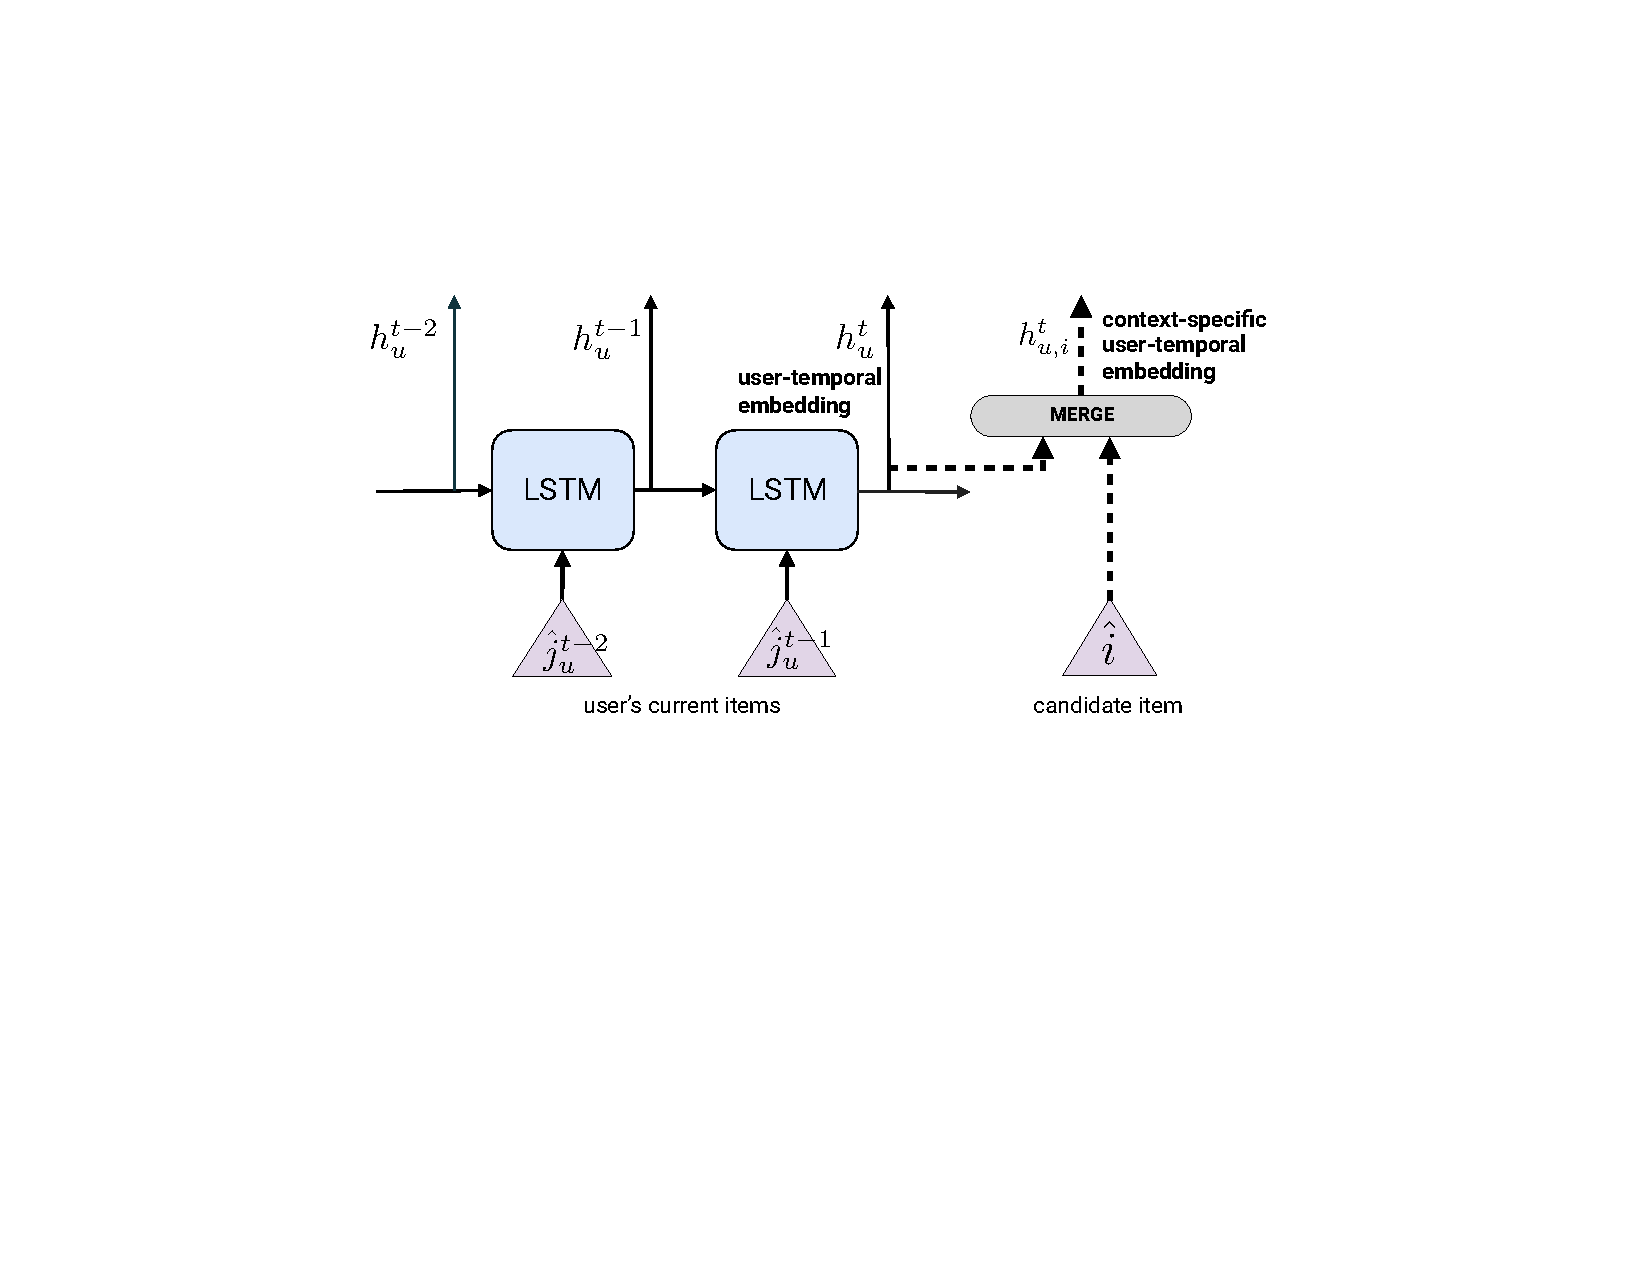
\includegraphics[width=0.7\textwidth]{figures/Temporal_new}
\caption{The user-temporal module uses an LSTM to compute an embedding $h_u^t$ based on a user's history $h_u^{t-1}$ and the current item $\hat{j}_u^{t-1}$. We also compute context-specific user-temporal embedding $h_{u,i}^{t}$ with respect to  candidate item $i$.}
\label{fig:temporal}
\end{figure}

\begin{figure*}[tbh]
\begin{subfigure}[c]{\linewidth}
\centering
  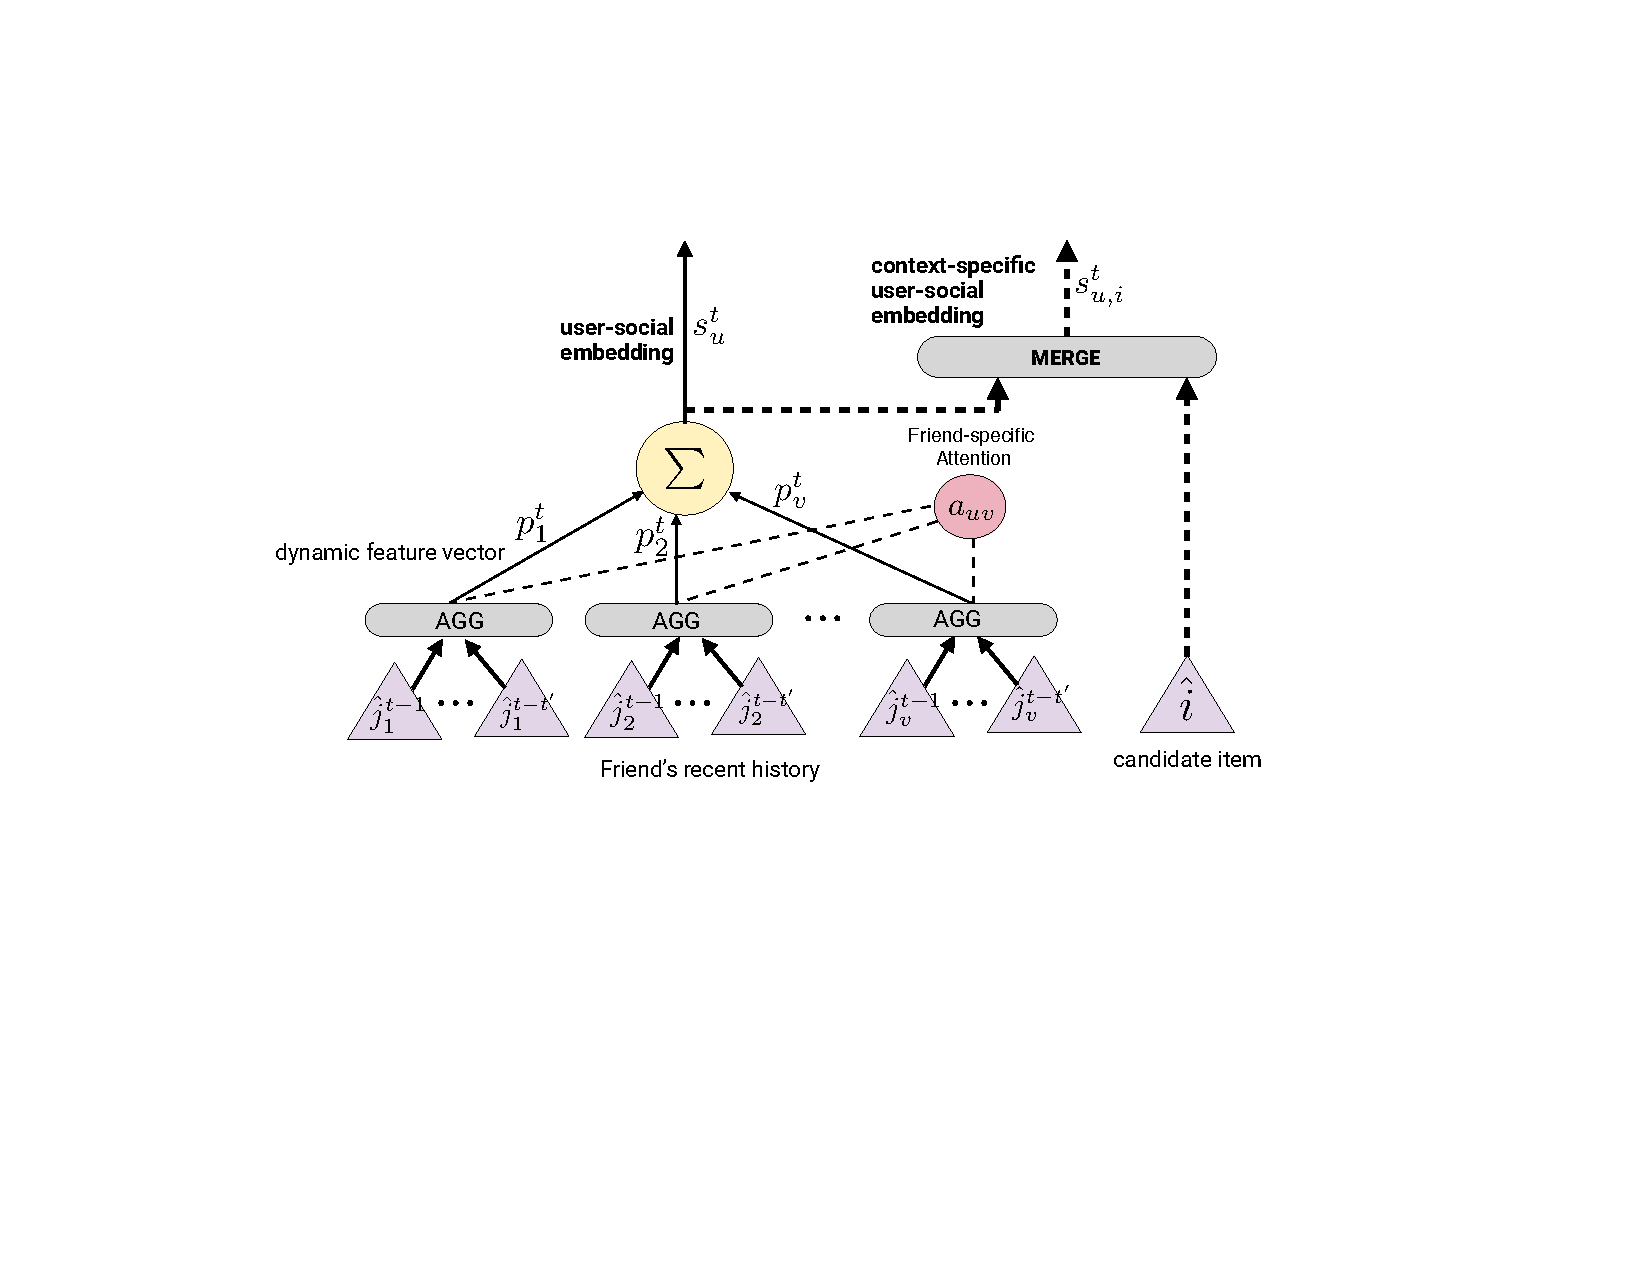
\includegraphics[scale=0.75]{figures/UserSocial_new}
  \label{fig:user}
\end{subfigure}
\caption{Illustration of the user-social module. The user-social module uses an attention based aggregation of the recent history of a user's social connections.}
\end{figure*}

\begin{figure*}[tbh]
\begin{subfigure}[c]{\linewidth}
\centering
  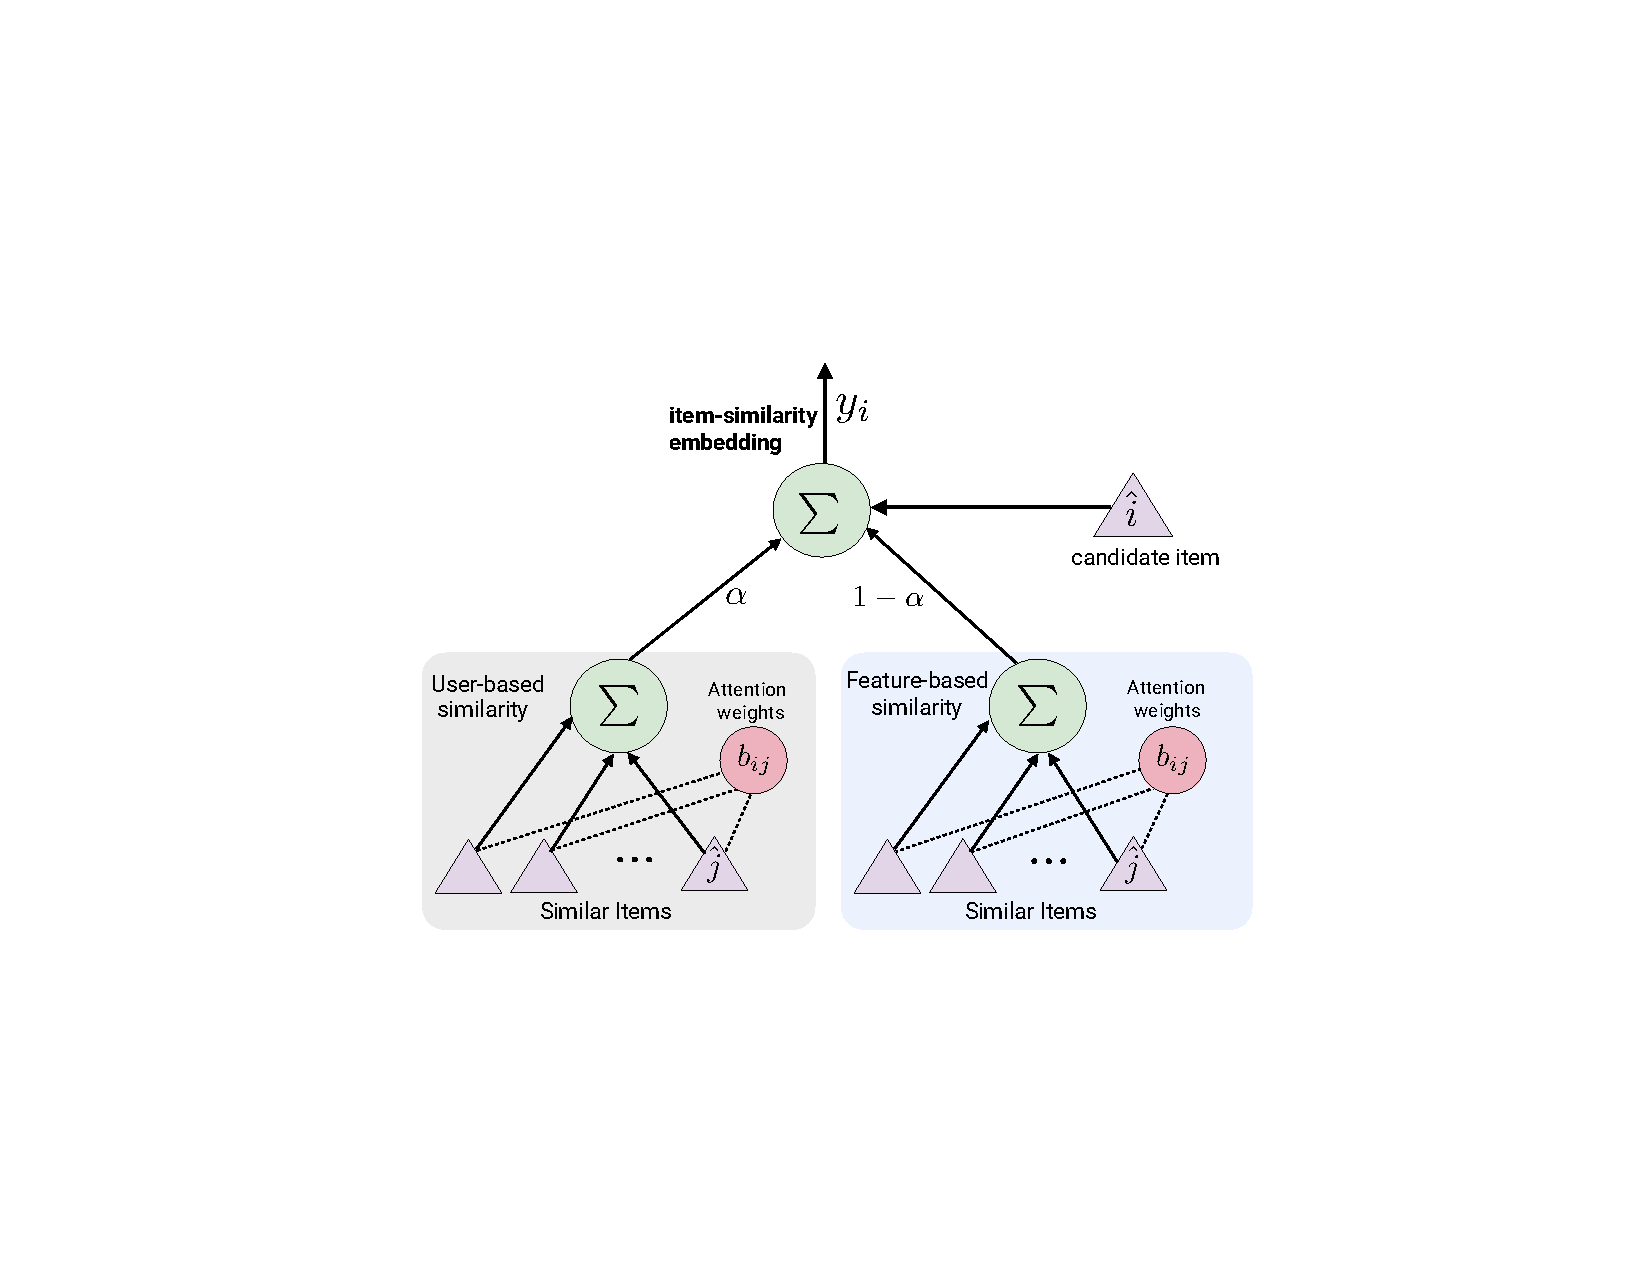
\includegraphics[scale=0.75]{figures/ItemModule_new}
  \label{fig:item}
\end{subfigure}
%\vspace{-0.2in}
\caption{Illustration of the item-similarity module. The item-similarity module aggregates embeddings from similar items in an attention aware manner. The item graphs are constructed based on frequency of co-occurrence and feature similarity. The parameter $\alpha$ trades influence between both item social graphs.}
\end{figure*}

\subsection{User-Temporal Module}
Users constantly interact with items offered on online platforms, e.g., users rate or watch movies. Importantly, a user's preference does not remain constant and changes over time.
To model temporal dynamics, classical methods have explored Markov chains, attention networks and convolution networks~\cite{FPMC, SAS:2018, Caser}. However, these methods assume dependence on only recent history and  thus do not capture long term dependencies within user-item preferences. To address this concern, we  use recurrent neural nets (RNNs) based on long-short-term-memory (LSTM) components. Those are widely used in natural language processing to capture sequential dynamics \cite{recurrent}.

In general, RNNs are based on the following recurrence relation, where $h^{t}$ represents the hidden vector at time $t$, $x^t$ is the input at time $t$ and $w$ refers to learnable weights:
\begin{align}
  h^{t} &= f(h^{t-1},x^{t-1}, w).
\end{align}

To specialize to our case, consider again a platform where users watch movies.
Formally, for each user $u$ at time $t-1$, let $j_u^{t-1} \in {\mathcal I}$ be the item which user $u$ interacted with at time $t-1$.  To compute its item embedding $\hat{j}_u^{t-1}\in\mathbb{R}^D$ (throughout we use `$\hat\cdot$' to indicate embeddings), we concatenate the item $j^{t-1}_u$  with its one-hot category information $c(j^{t-1}_u) \in \{0,1\}^{|C|}$ and apply the linear transformation
\begin{align}
  \hat{j}_u^{t-1} &= W_p [ j_u^{t-1} \mid \mid c(j^{t-1}_u)] + b_p.
\end{align}
With slight abuse of notation $j_u^{t-1}$ also denotes the one-hot representation.
Here, $W_p$ and $b_p$ are trainable parameters and represent weight and bias of a linear layer, `$ \mid \mid $' represents the concatenation operation and $C$ is the total number of item categories. This item embedding $\hat{j}_u^{t-1}$ is used as an input for an LSTM module based RNN which computes the user-temporal  embedding $h_u^{t}$ via
\begin{align}
  h_u^{t} &=  f'(h_u^{t-1}, \hat{j}_u^{t-1}, w).
\end{align}
Here, $f'$ represents the LSTM recurrence relation. This final user-temporal representation encodes a user's past behavior.

While $h_u^t$ captures a user's current preferences in general, we also separately capture relevance of candidate item $i$ with respect to the user's current preferences. For instance, if the user is currently watching action movies, we should capture if the candidate action movie $i$ matches her preferences.
Thus, context-specific user-temporal  embedding $h_{u,i}^t$ encodes similarity between user-temporal  embedding $h_u^t$ and the candidate item embedding $\hat{i}$.  Specifically, to capture similarity between the user-temporal embedding and the item embedding,
we compute $h_{u,i}^t$ as
\begin{align}
  h_{u,i}^{t} &=  W_q[h_u^{t} \mid \mid \hat{i} \mid \mid h_u^{t} \otimes \hat{i}] + b_q,
\end{align}
where $\hat{i}$ is the embedding of candidate item $i$ and $\otimes$ represents an element-wise product of two vectors. $W_q$ and $b_q$ are learnable parameters. \Cref{fig:temporal} depicts the architecture of this user-temporal module.

\subsection{User-Social Module}
Beyond temporal changes, users are influenced by recent behavior or ratings of  trusted friends. Also, influences are not equal among all friends.
To model this heterogeneous social influence, we use an attention based aggregation of a user's friends recent past behavior.  \Cref{fig:user} shows our user-social module. Formally, for user $u$ at time $t$, the user-social embedding $s_u^{t} \in \mathbb{R}^D$ is computed as
\begin{equation}
  \label{eq:user}
  s_u^{t} = \sum_{v \in F(u)} a_{uv} p_v^t,
  \end{equation}
where $F(u)$ represents  social connections of user $u$, $a_{uv}\in\mathbb{R}$ is the attention weight for friend $v$ and $p_v^t \in \mathbb{R}^D$ is a feature vector representing the recent history of friend $v$.

Most of the social recommender systems \cite{SBPR, SERec, GBPR} employ a uniform weighting for all social friends when computing influence. However, we argue that this is sub-optimal, particularly for social media, where a user does not trust  all friends equally. Indeed, we think modeling of trust is particularly important for online platforms due to large social circles with  superficial acquaintance. Thus,
we obtain the attention weights $a_{uv}$ from an influence score $e(u, v)$ for each user $u$ and friend $v$:
\begin{equation}
  e(u,v) = \text{LeakyReLU}(W_q [\hat{u} \mid \mid \hat{v}] + b_q),
  \end{equation}
where $\hat{u}, \hat{v} \in \mathbb{R}^D$ are user embeddings for user $u$ and $v$ respectively, while $W_q$ and $b_q$ are learnable parameters. The  attention weight $a_{uv}$ is  obtained by normalizing the influence score via a soft-max:
\begin{equation}
  a_{uv} = \frac{\exp(e(u,v))} {\sum_{v \in F(u)} \exp(e(u,v))}.
  \end{equation}

Each friend $v$ is represented by a dynamic feature vector $p_v^t$ which captures recent past behavior and is computed via
\begin{align}
  \label{eq:useragg}
  \hat{j}_v^{t'} &= W_r [ j_v^{t'} \mid \mid c(j_v^{t'})] + b_r, \\
  p_{v}^{t} &= \operatorname{AGG}(\{\hat{j}_v^{t'} \mid t' < t \}).
\end{align}
Here $\hat{j}_v^{t'} \in \mathbb{R}^D$ is the item embedding for item $j_v^{t'}$ clicked by user $v$ at time $t'$. Each past item rated by the friend before the current timestamp $t$ can be used to compute the historical profile of  friend $v$. In practice, we found that using the recent past gives similar performance compared to using all previous items. Therefore, we consider only the last $t'$ items of each friend. We aggregate these historical item embeddings using the mean aggregation operation $\operatorname{AGG}$. Note that
it is possible to aggregate this information in multiple ways but mean aggregation performed well in our experiments. It is also worthwhile to note that attention weights remain static across time while a user's feature vectors are dynamic.

Similar to the user-temporal module, we also compute a context-specific user-social embedding $s_{u,i}^t$. This embedding captures similarity of the user's social preferences with respect to the candidate item $i$. Formally,
\begin{align}
  s_{u,i}^{t} &=  W_s[s_u^{t} \mid \mid \hat{i} \mid \mid s_u^{t} \otimes \hat{i}] + b_s,
\end{align}
where $\hat{i}$ is the item embedding of candidate item $i$ and $\otimes$ is the element-wise product.

\subsection{Item-Similarity Module}
Online platforms operate with a large set of items, many of which are rated infrequently. It is consequently hard to construct meaningful representations of items, particularly if available information is scarce. Also, users are similarly attracted to related items but it is non-trivial  to implicitly learn item-item similarity.
To address this concern, we propose to construct a similarity aware item embedding based on information available for users which have interacted, e.g., clicked this item, and item features like category information.  \Cref{fig:item} illustrates our item-similarity module.

In particular, we represent each item $i \in {\mathcal I}$ via an n-hot vector $g_i \in \{0,1\}^{\vert \mathcal{U} \vert}$, where $n$ is the number of users who have interacted with item $i$ while $\vert \mathcal{U} \vert$ is the total number of users on the platform.  We then compute $k$-nearest neighbors for each item using cosine similarity between these n-hot vectors. This results in an implicit social network for item $i$, denoted by $F(i)$. All these items are similar as the same users interacted with them.
However, this approach of computing similarity between items is biased towards popular items with high user degree. Thus, we construct another item similarity network based on item features. In particular, we compute the  network $F' (i)$ based on items which belong to the same category.
We randomly connect $k'$ items of the same category in $F'(i)$. In our experiments, we let $k = k' $, i.e., we use the same neighborhood size for both  item networks.

We then  aggregate both of these item  graphs to learn item-similarity embeddings via
\begin{align}
  \label{eq:item}
y_i = \alpha \sum_{j \in F(i)} b_{ij} \hat{j} + (1-\alpha)\sum_{j \in F'(i)} b_{ij} \hat{j} + \hat{i},
\end{align}
where $\alpha\in[0,1]$ is a learnable parameter which controls the effect of co-occurring similarity versus category relationship. To compute the attention weights $b_{ij}$, we follow our earlier approach:
similar to the user model, $e(i, j)$  is the influence score for each item $i$ and its similar item $j$:
\begin{equation}
  e(i,j) = \text{LeakyReLU}\left ( W_n\lbrack \hat{i} \mid \mid \hat{j} \rbrack + b_n \right),
  \end{equation}
where $\hat{i}, \hat{j}$ are item embeddings for item $i$ and $j$ respectively, and $W_n$ and $b_n$ are learnable parameters. The final attention weight is obtained by normalizing the influence score via a soft-max function:
\begin{equation}
  b_{ij} = \frac{\exp(e(i,j))} {\sum_{j \in F(i)} \exp(e(i,j))}.
  \end{equation}
Note that we use the same embeddings to compute attention weights for both graphs.

The final estimated `item-similarity' module models similarity between items with similar features and frequently co-occurring items. This helps to address the data sparsity in the item space by exploiting item homophily.


Each module learns separates factors which influence user choices in recommender systems. We fuse these factors via a linear operation as detailed in Eq.~\eqref{eq:fuse}.

\subsection{Training}
We train all the three modules jointly in a unified framework using the binary cross-entropy loss:
\begin{equation}
L_{\theta} = - \sum\limits_{(u,i,t) \in \mathcal{B}}r_{ui}^t \log \left( \hat{r}_{ui}^t \right) + \left ( 1-r_{ui}^t \right ) \log \left ( 1-\hat{r}_{ui}^t \right) ,
\end{equation}
where $\theta$ represents all the learnable parameters in the model and $\mathcal{B}$ is the currently sampled mini-batch.
Specifically, for each sample $(u,i,t) \in \mathcal{B}$, we also obtain user $u$'s friends, $F(u)$ along with the corresponding item graph of the item $i$, i.e., $F(i)$ and $F'(i)$.

As we are dealing with implicit feedback, we don't have any negative samples. Thus, in each iteration of the training process, for every observed user-item interaction at time $t$, $(u,i,t) \in \mathcal{B}$, we sample $m$ unobserved items for user $u$.
Similar to \citet{Song:2019}, we assign a weight of $1/m$ for each negative instance to provide a weak negative signal. This is done as each unobserved item does not necessarily mean that the user will not interact with this item in the future. For our experiments, we set $m=5$.

\noindent
\textbf{Parameter Settings.}
For all three modules, we use an embedding size $D = 32$ for all user and item embeddings. We also initialize the embedding matrix using a Gaussian distribution with a mean of 0 and a standard deviation of $0.01$. For the user-social and item-similarity modules, in each iteration, we subsample a set of friends $F$ at each timestamp for a user (item) instead of considering all friends. This sampling has two benefits: (1) it avoids overfitting by introducing random noise in the social module; and (2) it is computationally more tractable. We use a sample size of 10 for both user $F(u)$ and item $F(i), F'(i)$ social graphs. If a user has less than 10 friends, we pad the remainder with zeros. We set a friend's past history length, $t' =  3$ in the user-social module. We will study the effect of this  and other hyper-parameters subsequently.

For the user-temporal and user-social module, we set the length of the historical sequence of user interactions to $30$ for all users. For users with history length less than $30$, we utilize all the available interactions.
We also study the effect of this sequence length on our results in the next section.
We use the Adam optimizer for training our model and perform a grid search over \{0.1, 0.01, 0.001\} for a suitable learning rate on the validation set. We report results on the test set for the best performance model on the validation set. We also use dropout along with gradient clipping with a value of 0.25 and L2 regularization on the user and item embeddings to avoid overfitting.
